\chapter{EA}\label{chap:EA}

\minitoc


%%%%%%%%%%%%%%%%%%%%%%%%%%%%%%%%%%%%%%%%%%%%%%%%%%%%%%%%%%%%%%%%%%%%%%%%%%%%
%%%%%%%%%%%%%%%%%%%%%%%%%%%%%%%%%%%%%%%%%%%%%%%%%%%%%%%%%%%%%%%%%%%%%%%%%%%%
%%%%%%%%%%%%%%%%%%%%%%%%%%%%%%%%%%%%%%%%%%%%%%%%%%%%%%%%%%%%%%%%%%%%%%%%%%%%
\section{Chronologies of the evolutionary algorithm }
%\chapterintro
%The genetic and biology has given rise to the evolutionary algorithm family in computer science.  
\chapterintro*{T}he evolutionary algorithm (EA) is a big family of algorithm and they included many meta-heuristic used in the field of optimization and artificial intelligence.\\
 The evolutionary algorithm are inspired by the biologic mechanism for design meta-heuristics. The origin of the inspiration can be varied as  the genetic, insect work, animal behavior, … (see Table  \ref{tab:EAlist}). \\
 The biologic inspiration are not the only elements use to define the evolutionary algorithms. All the algorithms in this family are dedicate to optimize iteratively a population of solutions. 
 The EA family are not deterministic and use a randomised function in order to evolve. \\
 To summarize the EA have most of this attribute : 
\begin{description}
\item Bio inspired. 
\item Use random (not fully deterministic).
\item Based on population. 
\item Evolve a set of solutions to optimise a problem.
\end{description}
These characteristics are not the strict definition for all the EA. They are rather the most common element of the major part of the vast EA family. The EA family include several  sub-categories as in Table \ref{tab:EAlist}. In the following  part the EA is approach more in details,  first a brief historic of the EA. 
 
 
 \begin{table}
   \begin{tabular}{ | m{0.35\linewidth} | m{0.35\linewidth} |  }
     \hline
      \Emph{Inspiration or group}   & \Emph{ Algorithm}    \tabularnewline \hline 
	  Based on memorization. & Neural network 				  	    \tabularnewline \cline{2-2}	
	  						 & 	Learning classification		 		\tabularnewline \hline 
	  Animal inspired and swarm algorithms & Particle swarm optimization (PSO) \tabularnewline \cline{2-2} 
	  				  		 & Bee colony 					  	    \tabularnewline \cline{2-2} 
	  				  		 & Ant colony 					 	    \tabularnewline \cline{2-2}  
	  				  		 & Mimetic algorithm			  	    \tabularnewline \cline{2-2}  
							 & Shuffle frog					  	    \tabularnewline \hline  
	Swarm algorithms		 & Addaptatif dimensional search  	    \tabularnewline \cline{2-2}  
							 & simulated annealing			  	    \tabularnewline \hline  
	  Combinatorial      	 & Harmony search 				 	    \tabularnewline \hline
      Genetic  				 & Genetic programing 		 	  	  	\tabularnewline \cline{2-2}
      						 & Evolutionary programing 	  	  		\tabularnewline \cline{2-2}
      						 &	Evolutionary strategies  	  	 	\tabularnewline \cline{2-2}
      						 &	Evolutionary programing 	 	  	\tabularnewline \cline{2-2}
      						 &  Genetic Algorithm			  	    \tabularnewline \hline  
   \end{tabular} \caption{Liste of few basic EA } \label{tab:EAlist}
 \end{table}
 
%\begin{table}[!htb]
%\begin{tabular}{|l|l|l|l|l|l|}
%  \hline
%  \multicolumn{2}{|l|}{z=1 } &\multicolumn{2}{|c|}{GA}  & \multicolumn{2}{|c|}{PSO} \\  \hline
%  \multicolumn{2}{|c|}{ } & GT & NW & GT & NW\\ \hline
%  Room &  120x80 & 16 &20 & 16 & 20\\ \cline{2-6}
%     &  240x160 & 64 &70 & 64 & 70 \\ \hline
%  Room U &  120x80 & 12 &20 & 12 & 20\\ \hline
%  \multicolumn{2}{|l|}{z=2 } &\multicolumn{2}{|c|}{GA}  & \multicolumn{2}{|c|}{PSO} \\  \hline
% Room &  120x80 & 4 &10 & 4 & 10\\ \cline{2-6}
%     &  240x160 & 16 &20 & 16 & 20 \\ \hline
% Room L&  120x80 & 3 &10 & 3 & 10\\ \cline{2-6}
%     &  240x160 & 15 &20 & 15 & 20 \\ \hline
%\end{tabular}
%\caption{Design of experiment for comparing the efficiency of PSO and GA in different conditions.  (GT is Ground Truth and NW is Number of Waypoints).}\label{table:table1}
%\end{table}

%%%%%%%%%%%%%%%%%%%%%%%%%%%%%%%%%%%%%%%%%%%%%%%%%%%%%%%%%%%%%%%%%%%%%%%%%%%%%
\subsection{ Fast historic of EA }

The EA are relatively young  and do not have one fix origin. It is the result of more than a decade of research and improvement.
The premise of the EA can be the work of Robbins et al  \cite{184*robbins1951} in 1951. 
More commonly, the beginning of the EA are on the late 50s with the works of Bremermann \cite{185*bremermann1962}, Friedberg \cite{186*friedberg1958}, Box \cite{187*box1957}. They propose different algorithms base on the evolving solutions to optimize a problem.\\ 
During almost the three next decade, the research had slowly progressed and they have remained rather unknown. Mostly due to the lower computation power at this time and also to some methodological short comings of
those early approaches. \\
Instead this difficulty, the fundamental works of Holland \cite{111*Holland1962}  and Fogel  has been essential to the progress and to popularize the EA. \\
As of 90s, due to the fast increasing computation power the EA became more popular and numerous new algorithms form EA family have been designed  as listed in the Table \ref{tab:EAlist}. The application of the EA in the engineering field (examples in \cite{10in182*alander1994}) and the multiplication of the conference around EA allowed the democratization of these family of algorithms.\\
The EA  has been profit of three main and independent methodologies; evolutionary programming, evolution strategies and genetic algorithms (GA). 

\begin{itemize}
\item The evolutionary programming, especially the work of Fogel is based on the finite state machine. The goal is to predict events based on the inputs, it is one of the premises of machine learning and classification.\\ %  sur les machine  a état fini (finit state machine ) ce sera les prémise de l'aprentisage

\item The evolution strategies, especially the work of  Rechenberg (\cite{rechenberg1965}), which propose a strategies based on deterministic selection and random mutation. The goal was to solve difficult experimental problem with discrete or continuous search space. \\ 
%strategies composé de mutation aléatoire et de slection deterministe  plutot destiner au espace continue et discret

\item The genetic algorithm is the most probably the most polyvalent and diversify of the EA (in terms of algorithm mechanisms). The GA propose  an adaptive processes to optimize a solution. The detail of GA mechanism will be explained precisely in the Section \ref{sec:GA}.\\  
\end{itemize}

%finir le résumé  pour  evolutionary programing   et evolution strategie 
The GA has more particularly attracts the interest of the research with the work of Holland and  Goldberg. The popularity of the GA is most probably due to the increasing power of computation (in 80s, 90s) associate to fundamental progress and the numerous possible applications in the optimization field.

Since the late 90s the research of EA have been focused on the multi objective evolutionary algorithms MOEA   \cite{75*zhou2011, 114*Zhang2007, 140*soremekun2001}. %and MOEA/D = MOEA cut in subproblem



 
%%Wiki source 
%%Evolutionary programming was introduced by Lawrence J. Fogel in the US, while John Henry Holland called his method a genetic algorithm. In Germany Ingo Rechenberg and Hans-Paul Schwefel introduced evolution strategies.
%%a lire


%%%%%%%%%%%%%%%%%%%%%%%%%%%%%%%%%%%%%%%%%%%%%%%%%%%%%%%%%%%%%%%%%%%%%%%%%%%%
\subsection{ General formulation of  EA. }\label{sec:GeneralEAform}

 The EA is vast and many type of algorithms exist in this family, despite that a global formulation is proposed.\\
 Most of the EA have to optimize one or several problems using an iterative process to evolve towards a best solution. The EA can be formulated as the optimization of a parametres vector. Where each element of the vector ($\vec{x}$) is one input or a dimension to optimize. \begin{equation}
	\vec{x}= \{x_1,...x_n \} \in \omega
\end{equation}
Where $\omega$ is the search space of the problem, $n$ the number of dimension to optimize(or number of input). Each dimension of $\vec{x}$ must have a limited range (as $ \sum^{n}_{i=1} \sup x_i \leq x_i \leq \inf x_i$ ).  The search space represents all the possible solution of a problem. \\
In the case of the elements in the vector $\vec{x}$ are ordered, the search space even bigger. In this case, it is the product of each range of the vector.% ( as $ \prod^{n}_{i=1} \sup x_i \leq x_i \leq \inf x_i$ ). 
Where $||x_i||=\sup x_i -\inf x_i $ it is range size of  $x_i$ thus the size of the search is define as  $ \prod_{i=1}^{n} ||x_i||$. \\

Thus, the search space of the problem is defined by the boundary of each dimensions and the number of dimensions.  
%The association of each limitation for each dimension, define the search space of the problems( The boundary of the solution).
 Bigger is the search space, more the solution may be long to find in term of computation and power complexity.

 The goal of the EA family is to optimize inputs ($\vec{x}$ in order to have the best solution possible for the problem. Where the best solution is defined by a cost function depending than the input a vector $f(\vec{x})$. 
\begin{equation}
	\max f(\vec{x})\leq f(\vec{X})
\end{equation}
 Where  $\vec{X}$ is the global optimum solution. \\
 The cost function $f(\vec{x})$  is unique for each problem and have to be redesigned for  each problematic. 
Depending then the problem, the global solution is unknown and the best is to tends to this supposed global optimum solution. 
Optimize a solution $\vec{x}$ is not always enough to solve efficiently the problem. 
The solution proposed have to respect the constraint linked to the problem. The constraint can be various depending than the problem. As example one naive constraint is the boundary of the search space. To reach a set of $m$ constrain $E$ must be taken in consideration.
% But optimize a solution $\vec{x}$ depending on the fitness function is not enough to reach to the global optimized solution $\vec{X}$. To reach it a the set of $m$ constrain $E$ must be taken in consideration.
\begin{equation}
 \begin{split}
	\min (\sum^{m}_{j=1} e_j(\vec{x} ) )=E
    \\
	\max F(\vec{x}) \forall \vec{x} \in E 
  \end{split}
\end{equation}  
 $F$ is the final cost function, with include the constraints, to evaluate a solution $\vec{x}$ to optimize the problem. \\
The EA manage the optimization of the problem based on the cost function $F(\vec{x})$ by applying different meta-heuristic. 
The meta-heuristic use different methodologies to optimize an initial solution. The optimisation is more or less global depending than the method chosen. 
Mainly the optimization methods are based on the generate new sets of solutions. The new sets is made by evolving the previous sets of solutions. A set of solutions is also called population. %try to optimize an initial solutions based on the generation of a population of solutions. 
Where  a population is defined as $pop=\{\vec{x_1}, ...,\vec{x_p}  \}$ with $p$ is the number of individual in the population. 
%The EA are not obviously use in the convex problem 
The solution found by the EA is not mandatory the global optimum and for some type of problem (as Np-hard) it is impossible to confirm it. \\
The risk in this case is to try to optimize indefinitely. Instead to control the end of the optimization a stopping criteria  need to be taken in account.
%Instead to control the end of the optimization for do not indefinitely loop, a stopping criteria need to be taken in account. 

\subsection{Stopping criteria and convergence}
% \paragraph{Stoping criteria. // a deplacer dans le GA ou pour les algo de type GA PSO memetic ant}
 
The EA does not provide a solution to decide when is necessaries to stop the optimisation. 
To control the stopping criteria different solutions exist. The solutions proposed in the following part are mostly adapted to the algorithm like GA, PSO, mimetic and other EA working with a population to optimize.


% Therefore even if the global optimal solution is reached it is impossible to be assured of it. 
The EA algorithms are mostly efficient in the problems with many local minima. Due to numbers and size of the local minima it can be difficult to assure if a solution is the best or more exactly the global optimum. 
To know if the global optimal is reached, the method must be sure which no other solution can be the better. Therefore the solution found must be always exactly the same or equivalent in term of cost. The optimisation process must be reproducible (same input gives the same output).\\
 Only the deterministic method can insure to have a global optimum solution as a convex problem. The convex problem has only one global optimal and no local minima. \\% Using a algorithm from the EA family do not authorize such insurance due to the randomness effect proper to the EA.\\ %manly due to the impossibility to reproduce every time the same result in the same condition due to the randomness effect proper to the EA family.
  In this case, the EA looking for the better solution possible (not the optimum). That can be in some case the same then the global optimum but because of the uncertainty is impossible to call global optimal it is just the better solution founded.  
 
% methode non deterministe donc imponsible de connaitre la solution optimal donc commen sarrété.
%How to know if a solution is the better solution and related to
%In many case the optimal solution cannot be reach and a stopping criteria should be defined. Manly 3 possible way are communally use.

Based on that, how  determine when is time to stop the optimisation with EA. At some point is useless to continue the optimization (best solution founded or lock in some deep local optimum) and a stopping criteria should be defined.\\ 
Three possible way are communally used:\\
\begin{itemize}
\item The first method (called fix time criteria), is to stop the optimization after a fix numbers of iteration or time limit. The limit is measured in term of time computing, also the numbers of iteration must be fixed by the user. The interest of this method is manly to control the time of computation for the problem requiring a solution in a determined time (as a real time). The risk of this method is to stop the optimization before to have an efficient solution. \\
This solution can be mixed with other method to reduce the number of useless iteration.% for control the case where the  other method are too long.  

\item The second method (called update criteria), is to stop the optimization (before the convergence) if no better solution is found after a predefined number of iteration. This criteria can be useful for the complex problem or if many solution can have the same quality. 
The advantage of this solution is to can stop before the convergence with a close solution. The inconvenient is to stop too early, in the beginning of the optimisation due to a good initial solution.   \\
To use this stopping criteria a correct number of iteration has to  be selected. 
The number of iterations  must be sufficient to give time when the meta-heuristic is lock local minima. 
A long time lock in local minima may append mostly at the early time of the optimisation due to the too good initialisation or in the late optimisation time (when the solution is already well optimized).\\
 In contrary a stopping criteria with a too big number of iteration became use less. In the worst case, the convergence point will be reached  before the too big number of iterations.
%si la meilieur solution est pas ammélioré 

\item The third method, (convergence criteria), is to stop the optimization by waiting the convergence point. The convergence is reach when the actual population is composed by a set of solutions identical. That means the same solution has been founded by all the individuals of the population. \\
 The best solution found  push the other to evolve in the same  direction, by contagion  all the individual  of the population evolves to reach the convergence point. \\ 
 This solution found during the optimisation process is supposed to be the better. In this case, the population has been converge to an optimized solution. At least no better solution can be found during this optimization.\\
\end{itemize}
This 3 criteria are the more commune, but depending the problem other criteria can be found with more or less a priori on the problem.\\

 Moreover the stopping criteria presented can be a combined to have an efficient and flexible solution as  in the following example :\\
The mixed stopping criteria is to combine a fix time criteria and the update criteria.
The advantage of the fix time criteria is to avoid the case of an almost infinite optimisation loop append, due to an impossible convergence.%(which leave a good room for manoeuvre to reach the convergence), 
\\ %The fix time criteria is fix widely to leave the manoeuvre to reach the convergence. \\ 
Combined with the update criteria the other advantage is to can stop the optimisation before the convergence and before to reach the time criteria limit.\\
The combination of these stopping criteria assures to have always a solution optimize in a reasonable time (fast, efficient and time predictable for the worst case). 

% Tout la population a la meme solution
 
%%%%%%%%%%%%%%%%%%%%%%%%%%%%%%%%%%%%%%%%%%%%%%%%%%%%%%%%%%%%%%%%%%%%%%%%%%%%%
%\subsubsection{ Relation enter Darwin et EA  }
%
%%%%%%%%%%%%%%%%%%%%%%%%%%%%%%%%%%%%%%%%%%%%%%%%%%%%%%%%%%%%%%%%%%%%%%%%%%%%%
%\subsubsection{ Historique des EA   }


%%%%%%%%%%%%%%%%%%%%%%%%%%%%%%%%%%%%%%%%%%%%%%%%%%%%%%%%%%%%%%%%%%%%%%%%%%%%
%%%%%%%%%%%%%%%%%%%%%%%%%%%%%%%%%%%%%%%%%%%%%%%%%%%%%%%%%%%%%%%%%%%%%%%%%%%%
%%%%%%%%%%%%%%%%%%%%%%%%%%%%%%%%%%%%%%%%%%%%%%%%%%%%%%%%%%%%%%%%%%%%%%%%%%%%
\section{Darwin and the natural selection }

The theory of evolution was introduced by Darwin and inspired the computer science for developing optimization algorithms. To understand the algorithm is important to go back to the origin.
%%%%%%%%%%%%%%%%%%%%%%%%%%%%%%%%%%%%%%%%%%%%%%%%%%%%%%%%%%%%%%%%%%%%%%%%%%%%
\subsection{Darwin theroy } \label{sec:GA}

Darwin has studied the differences between individuals from the same species and tried to establish a classification of the different sub-species. It appeared some individual animals from the same species and from different countries had some small differences. These variations were studied and explained by the Darwin theories in The Origin of Species, published in 1859. 

The origin of species details what will be called the theory of evolution. 

This theory uses the concept of adaptation introduced presciently by J.B. de Lamarck, and deeply studied by Darwin. The adaptation explains the relation between the environment of the individual and the differences generated by natural selection. This observation was first made on bird, called geospiza, or finches, (chaffinch) from Galapagos archipelago. Darwin noticed the difference of their beaks (see the Fig \ref{fig:finchesFromGalapagos}). The shape of the beak was correlated of the specificity of each island. Finches with the biggest beak correspond to the island with the biggest seed. \\
This observation was formulated and explained by Darwin by the adaptation of the bird in their environment.\\ The adaptation is partially due to the natural selection. Indeed the selection is done by the reproduction of the strongest individuals.\\
The reproduction concerned 2 individuals (one male, one female). Each individual is in competition with the other individuals of the same species.  In its condition only the stronger and  the more adapted individuals   have a chance to have a progeny (an offspring). In fact generation, after generation, the more adapted individual itself reproduced and mute, while the species adapt to their environment.
In this case, the strongest finches is the one with an appropriate beak in order to eat more seed. \\


\begin{figure}[t!]
\minipage{0.85\textwidth}
   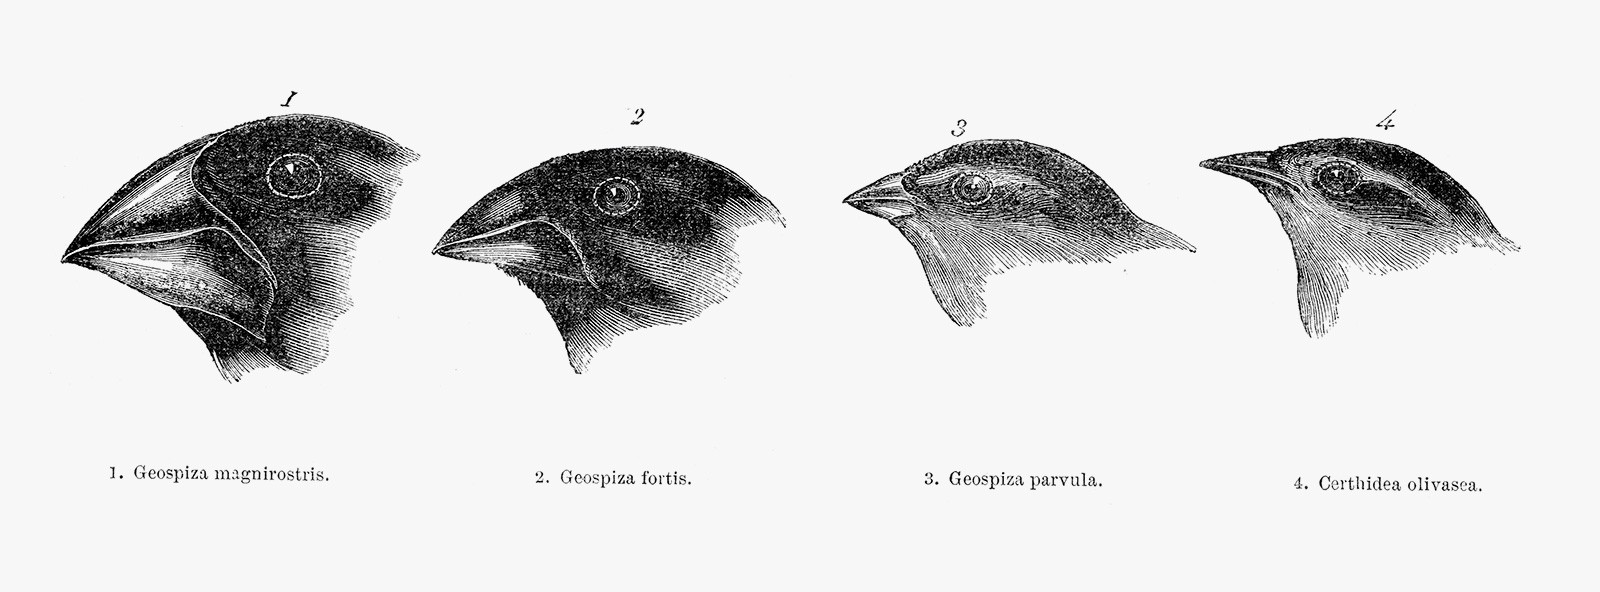
\includegraphics[width=\linewidth]{img/finchesFromGalapagos.jpeg}
  \caption{ Finches from Galapagos archipelago extract od The Origin of species by C.Darwin .}\label{fig:finchesFromGalapagos}
  \endminipage\hfill
\end{figure}

%%%%%%%%%%%%%%%%%%%%%%%%%%%%%%%%%%%%%%%%%%%%%%%%%%%%%%%%%%%%%%%%%%%%%%%%%%%%
\subsection{Biologic evolution }\label{subsec:BioEvolv}


The Darwin theory was validated, especially with the genetic progress. The progress in this field was used to study the mechanism of the natural selection and evolution. One of the important progress and confirmation of the theory is by using the analyse of DNA code.     \\
The discovery of DNA code permits to confirm the genetic proximity between  some species. Moreover the DNA permit to evaluate their evolution and code modification in the same species from different location and several generation gap. %voir eventuelement  l’évolution des petit lezar sur 20generation
Also the genetic may explained deeper and clearly the evolutionary process. 

\subsubsection{Biologic evolution process.}

In the biologies, every living element is composed by cellular. Inside each cellular  the DNA code is stoked. The DNA composes the chromosomes. The chromosomes have a central role in the definition of one individual and in the reproduction process (see the Fig \ref{fig:celTokrom}). \\
\begin{figure}[t!]
\minipage{0.85\textwidth}
   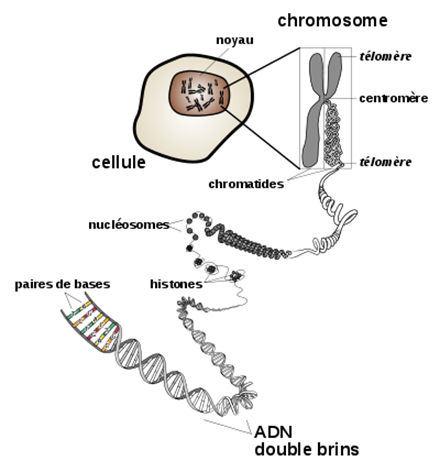
\includegraphics[width=\linewidth]{img/celTokrom.png}
  \caption{ Finches from Galapagos archipelago extract od The Origin of species by C.Darwin .}\label{fig:celTokrom}
  \endminipage\hfill
\end{figure}
As has introduced earlier, the evolution is possible by a natural selection. The selection is done by survival and reproduction ability of the better individual. Better mine more adapted to this environment, like for the geospiza the size of the beaks depending than the size of the seed from his island.
In the island with the big seed  the geopiza with the small beaks was not the more adapted and have more difficulties to find food. This weakness make the geopiza with the bigger beaks in better position to reproduce and the DNA of the individuals with biggest beak is transmit at the next generation.\\
 The understanding of the reproduction mechanism in term of succession and transfer of the natural ability is primordial. It is explained in part by crossover in the cellular state.
 %sexual reproduction 
 \subparagraph{Sexual reproduction. }
The living element for example the geospiza use sexual reproduction. The sexual reproductions assume to merge  part of the chromosome form the two individuals to create their descendants. The selection is essential in order to keep the more adapted individuals of the species. \\ 
Among the reproduction mechanism the crossover and the mutation are the one with the bigger impact.
%% crossover
\subparagraph{Crossover. }
The crossover is the action of merging the chromosome of two individuals in order to have a new child.\\
It is an essential factor to preserve the individual ability of the geospiza. But the natural section and the crossover cannot be considered as the only useful element to evolve. 
%genome
\subparagraph{Genome}
The genome is a subset of the DNA code. Communally the DNA is cut in many thousand genome where each genome can represent a specified function or ability.  
%% mutatoin 
\subparagraph{Mutation. }
%The mutation is another essential element of the evolution process. 
Instead of the crossover which allows only the ability preservation from one generation to another, the mutation introduces some “anomalys”. The anomaly can become in some case a biologic advantage.
The mutation affects only rare chromosomes of the individual. The chromosomes affected are not fully mutated but only one or two genomes are affected. \\
%The genome is a subset of the DNA code. Communally the DNA is cut in many thousand genome where each genome can represent a specified function or ability.  
The mutation changes the little piece of DNA code to introduce variety in the genetic code by the small “anomaly”.\\
Most of the time the small mutations are not consequent for the individual but generation after generation the mutation can be preserved and spread in the population. \\  



The giraffe can be taken in example:\\
 In the arid environment, the giraffe with the longest neck has more chance to survive due to this empowered to find food. The giraffe with a neck a bit longer than the other, can became more attractive for the natural selection (in this case more food mean stronger and more attractive). The natural selection pushes the best individual to reproduce together and by the crossover mechanism conserves the small advantage given. The initial mutations give at few giraffe a longest neck and by the process of natural selection associate to the crossover allows this advantage form a small mutation to become the norm. Mutation by mutation and generation after generation the giraffe  saw the average length of their neck increased. Finally the actual giraffe is the result of a long and complex evolutionary process. \\ 
The mutation can also be the source of degenerate animals but in this case the natural selection  by the reproduction (and crossover) will not allow the preservation of the individual and thereby the mutated chromosome will disappear.\\ 

\section{ Genetic algorithms}
Among the evolutionary algorithms one of those was very close to the Darwin theory by reusing the operating principle of natural selection and was also based on the genetic with the influence of the crossover and mutation (see  section \ref{subsec:BioEvolv}). This algorithm is calling Genetic Algorithm (GA) and was introduced for the first time by Holland in 1962 \cite{111*holland1962}. \\
The genetic algorithm (GA) is from the EA family but is also one of the fundamental algorithms of the EA.
The GA became popular at the late 80s and early 90s, particularly with Goldberg works \cite{112*goldberg1989}. Many details were redefined and explored in the knowledge of genetics to have a huge set-up and operator available for the GA.

\subsection{GA evolution}

Whether GA is a relatively recent algorithm, it was largely studied during many years and has progressed tremendously. To follow the evolution of the GA  the survey  written in \cite{74*srinivas1994} for the Simple Genetic Algorithm (SGA) are a good point to understand the progress before 1994. 

In this article \cite{74*srinivas1994} the author begins to explain the SGA and the significance of the natural selection with the possible modification to adduce. 
Also the GA improvement  in term of performance is discussed. The SGA is parametrizable depending then the implementation. That give a big importance of the problem formulation and the consequences on the solution.
%Also the author discusses the research that have focused on improving GA performance including the distribution and the parallelization of the GA as well as the importance to encode properly the solution and the consequence on the solution. The encoding is the methodologies used to represent the parameters of the problem to optimize.\\  % a revoir ajouté les ref  de  l'article 
 This survey is  relatively hold (from 1994) and other more recent are rather focused on the Multi Objective Evolutionary Algorithms (MOEA), which include many different shapes of Genetic algorithms customized to satisfy the multi objective problems \cite{75*zhou2011}. \\
Although the papers are concerned about the multi objectives and many references are made to highlight the recent advance on this field with different types of adaptation. The evolutionary algorithm, like the multi objectives evolutionary algorithm decomposition (MOEA/D) \cite{114*zhang2007}. To decomposed the problem into sub-problems and each sub-problems are weighted by the neighbouring relation between the sub-problems then aggregated.  \\ 

It exists many other MOEA present in this paper as Non-dominated Norting GA II ( NSGA-II) \cite{69*deb2000} this  algorithm are using an elitist selection to optimize efficiently the problem without having to sort the different solution depending to the different objective. Some other MOEA as QGA for Quantum-inspired GA \cite{ 69*deb2000,han2000,han2002}%([146@, 147@])
, Non-dominated Sorting GA  (NSGA) or BMPGA for Bi-objective Multi Population GA [191]@,  are examined on this survey\cite{69*deb2000}. \\
The GA have been studied for different objective and optimization problem. these surveys  give a fast  view of  the GA formulation and  specific customization for  GA application field, as the following example.\\
% Some of this papers about it are presented in different survey article and can give a fast view of the specific customization of the GA and the field of application.\\

% from [75]
%[146]@ K.-H. Han, J.-H. Kim, Genetic quantum algorithm and its application to
%combinatorial optimization problem, in: IEEE Congress on Evolutionary
%Computation, CEC 2000, 2000, pp. 1354–1360.
%[147]@ K.-H. Han, J.-H. Kim, Quantum-inspired evolutionary algorithm for a class of
%combinatorial optimizati
%[191]@ J. Yao, N. Kharma, P. Grogono, Bi-objective multipopulation genetic algorithm
%for multimodal function optimization, IEEE Transactions on Evolutionary
%Computation 14 (1) (2010) 80–102.

\begin{itemize}

\item In \cite{117*sheikh2008} are interested on the problem of clustering and use GA for have a non-supervised clustering and also show the different implementation and customization of GA adapted to this problem. 
\item In \cite{ 122*wang1996}, the genetic algorithm is applied to the problem of pattern recognition. This problem is a complex multi optimization problem. The GA is used to optimize the classification, the training and the research of a set of efficient features. 
\item In \cite{ 123*owais2008}, the GA is applied to security problems to control computer access in the network and prevent attacks. In this case the GA can be used to optimize the classification of the access and this way detects the legal and authorized access then the hacking attempt.   
 
\end{itemize}

GA have been well studied  and the literature about is vast. These last decade the GA  has been used for multi objective problem but  its popularity has decreased in favour of algorithm which requires less configuration or other algorithm  more oriented on learning.  
%III GA explication   
 % Ga historique 
	%	SGA
	%	MOEA GA
	%	Utilisation du GA dans différent application
   
\subsection{Ga in detail}  

%After have seen in the previous part  the origin and some reference about the evolution of the GA.
In this section, the GA will be present with more interesting advance and set-up. 
The following section will try to list the more interesting aspects of the GA mechanisms. 

% It will not be a list of all the different implementations and mechanism, rather a detailed explanation that also gives the different optimization lists already explored or the more usual ones.  
 
 The explanation will be separated in 6 sections with:
\begin{itemize}
\item [1)] 	chromosome representation 
\item [2)]	population size 
\item [3)]	cost function 
\item [4)]	selection mode 
\item [5)]	operator 
\item [6)]	setting 

\end{itemize} 

Before beginning, it is important to remember the GA is an algorithm use to optimize a solution while still on a non-deterministic initiative and therefore can not give the certitude to have the optimal solution. 

\subsubsection{Chromosomes} \label{par:Chromosomes}
As in the Biologic field the chromosomes contain the properties (with the genomes and DNA) of the individual.
A primordial issue when you want to optimize a problem involving the GA is to define properly the chromosomes role, for that different aspects must be taken into account.\\

The first aspect is related to the problem himself. The chromosome is used to design the problem and it has to represent a solution. To do so, it is important to know the problem and identify clearly what parties of the problem need to be optimized and what is the range of the research area. \\
Depending on that the coding can be direct or indirect.
\begin{itemize}
\item The direct coding is code with the genomes corresponding to the elements of the solution. Using the direct coding may simplify the output of the optimization by returning it back to an element directly proper to use.
\item  In Contrary, the indirect coding, it is not directly proper to use and need conversion to be used. One example of indirect coding is the willingness to introduce redundant genome inside each chromosomes.  The conversion must be done by a heuristic. The interest of the method is to be able  to make a strong constraint adapted to the problem as \cite{ 121*ronald1997,131*walters1995}  where it is used to solve a complex scheduling problem with many constraints. 
\end{itemize} 
 Inside this article the interest between the direct and indirect coding are presented.  \\ %indirect ex metre de la redondence dans le chromosome
The diverse aspects of the problem should be clearly defined before the element makes up the chromosome, like  the number of dimension to optimize, the boundary of each dimensions and the importance of the dimension order. 
%!!!a finir verifier et surmen réecrire!!!!
When the chromosome is defined the second phase is to choose the best coding solution. Many solutions exist to encode the chromosome like presented in \cite{131*walters1995} and \cite{123*owais2008}   but among the coding solution, 4 main categories can be considered as  basic coding type,  which are the combinatory coding, binary, the real (also alphabet) and tree coding.

\subparagraph*{Binary Coding}(\cite{ 73*wright1991, 95*miller1995,97*goldberg1985,123*owais2008, 131*walters1995}).  
\\The binary coding offers to format the chromosomes as a bit string in which every genome of the chromosome can be covert on pack of bit with can have only 2 value 0 or 1. This coding method was studied since the beginning of the GA by Goldberg et al  \cite{97*goldberg1985} and also used in other EA like PSO in \cite{87*morsly2012}. The binary coding is more efficient in the small search space or when the size of the chromosome is not too long. The advantage of the binary coding is the possibility to introduce lot of variety during the process of optimization \cite{73*wright1991}. The variety is traditionally from the mutation but in the case of the binary coding the crossover introduce variety by the potential split of the genome in 2 pack of bit.
\\
\subparagraph*{The combinatory }(\cite{ 80*serpell2010,110*eiben2003} ).
\\The combinatory coding is commonly applied in some specific problems where the goal is to order all the element. In this case, the position of the genome in the chromosome is primordial as in \cite{ 110*eiben2003}. It is characteristically used to the problem as TSP \cite{80*serpell2010} (Travelling salesman problem).  When the combinatory coding is used for problem the aim is to optimize the order the element of the chromosome. With a combinatory coding the each chromosome already has all genome of the answer. An example, the TSP the aim is to order various cities (in the problem of TSP every genome represents a city) and all the possible cities are included in the initial solution (chromosome). In this case, the problem is to optimize the combination of the element composed by the initial solution. 
One evolution of the combinatory traditional coding is to can add and remove some genome, that obviously affect the size of the chromosome, for example  when the goal is to find the shortest distance in the tree \cite{113*mais2010}. \\

\subparagraph*{Real Coding }(\cite{ 73*wright1991, 123*owais2008,131*walters1995}).   
Real coding or integer coding is considering every genome of the chromosome as a number to optimize. This number can be a real or an integer and may have an infinity of possibilities in the negative or positive. In fact, the value does not have an infinity of possibilities because the constraint by the computer and limits of the problem itself too (size of the search space). This coding is used when the search space is large and also can be efficient when many dimensions need to be optimized. But most of the time a special attention should be put to the operator, because in many cases the operator may be adapted or redesigned depending on the problem such as in \cite{68*muhlenbein1989},  which the operators are adapted to look for close neighbours.\\
\subparagraph*{Tree coding }(\cite{ 113*mais2010, 123*owais2008, 131*walters1995}).   
The tree coding use the tree representation to take care of the hierarchy but this method is not really popular and not flexible to any case. The advantage of tree coding is this ability to go farer then a combinatory representation.  An example in \cite{131*walters1995}, the tree coding is used with the GA to optimize new network telephone or gas/ water pipeline where the relation between the element are primordial. In \cite{131*walters1995} present the interest of tree coding for  the intrusion detection system. 
\\\\
The 4 coding method presented are not the only potential coding, there are the more commune and the roots of other coding   and many other have been developed and studied with direct or indirect coding to feet  with specific problem. Thereby in the literature a survey are dedicated to the encoding chromosome for the GA \cite{121*ronald1997}. The survey \cite{121*ronald1997} propose to explain and find a robust coding usable depending then the problems. 
\\

%\begin{table}
%   \begin{tabular}{ | m{0.30\linewidth} | m{0.65\linewidth} |  }
%     \hline
%     \Emph{ Reference}   & \Emph{Chromosomes interest}    \tabularnewline \hline 
%	  Walters et al 1995 \cite{131*WALTERS1995} & Use the GA for pipeline position optimization with a tree coding and a talk about the choice of the coding compared to the binary coding and alphabet coding.  				  	    \tabularnewline \hline 
%	  						 & 	Learning classification		 		\tabularnewline \hline 
%      Genetic  []			 & Genetic programing 		 	  	  	\tabularnewline \cline{2-2}
%      						 & Evolutionary programing 	  	  		\tabularnewline \cline{2-2}
%      						 &	Evolutionary strategies  	  	 	\tabularnewline \cline{2-2}
%      						 &	Evolutionary programing 	 	  	\tabularnewline \cline{2-2}
%      						 &  Genetic Algorithm			  	    \tabularnewline \hline  
%   \end{tabular} \caption{Liste of few basic EA } \label{tab:EAlist2}
% \end{table}
%The variety is introduced due to the cutting pack of bit during the crossover. 



%[131*] codage par tree of GA codage par lettre alphabétique au lieux du binaire. 
%[121*] survey codage indirecte avec redondence 
%[123*] codage binaire and tree codage .  Use GA for security   ralk about the encoding chromosome  wihe  binary  permutaiton  real tree

%Parties détailler 
%1)	Comment représenter un Chromosome (individual) \\ 
%-	Codage Binaire (utilisé au début)
%-	Codage Réel  (plus adapté au problème  de variable  continue) 
%-	Codage combinatoires (pour les problèmes combinatoires) (à vérifier) 
%-	Tree coding
%
%2)	Fonction de cout :\\
%-	Importance de la fonction et universalité (même fonction pour tout les metaH)
%-	Multi objectif 
%-	Constraints (inside the cost function)
%-	Optimisation  and time computation 
%3)	Population \\
%-	population initiale  
%-	la rapidité de convergence  et variété 
%-	 taille de la population
%4)	Mode Sélection :\\
%-	Le rôle de la sélection 
%-	Elitiste selection
%o	Fonctionnent 
%o	Adaptation pour du MOEA
%-	Roulette wheel selection 
%-	Tournament selection 
%o	Fonctionnent 
%o	Taille de la poule 
%
%5)	Operateur  et leur fonctionnement\\
%-	Cross over
%-	Mutation
%-	Rate of operateur
%
%6)	Paramétrage : \\
%-	Liste de paramètre
%-	Leur inter relation 
%-	Configuration par test 




%%%%%%%%%%%%%%%%%%%%%%%%%%%%%%%%%%%%%%%%%%%%%%%%%%%%%%%%%%%%%%%%%%%%%%%%%%%%
\subsubsection{Cost function }\label{sec:CostFunctionGA}
	The cost function or some time called fitness function has an essential role in the optimization process.  The aim of this function is tantamount to quantify the quality of one solution. This point is primary to the GA and in most of the optimization process using meta-heuristic. The cost Function is an compass the meta-heuristic during the  optimisation. 
	The cost function is dependent then the problem and should be design or redesign depending on each specific  problem. Once the cost function is designed for a problem they can be used to test different other algorithms of optimisation with requires also a cost function. 
	Because the cost function is exactly the same that becomes easier to compare the results from different algorithms as is discussed in \cite{79*franccois2001} and also in the chapter \ref{sec:GAvsPSO}.%[GA VS PSO 5.2 ] 
	Once conceived the cost function is considered as a black box by the optimization algorithm and encloses most of the complexity of the problem. Obviously if the cost function is not designed correctly with all the constraints and the objective, the optimization will fail.\\

\paragraph*{Multi objectives}
The cost functions are traditionally made-up for  problems with only one objective, but in the recent years several solutions have been adapted for multi objective. The goal is to optimize a problem with few sub-objectives included. These sub-objectives can be at some point contradictory and a trade off must be done during the optimisation process, based on the rating made by the cost function. \\
 The cost function for multi objective problem (MOP) is discussed in the survey of Zhou et al \cite{75*zhou2011}. In Zhou et al \cite{75*zhou2011} one of the ways to solve the MOP is to adapt a classic mono objective algorithm in multi by customizing the cost function. The customization of the cost function propose a way to evaluate a solution not depending than one objective but with all of them combined in the same function instead of several cost function. 
 Also other solutions are discussed in \cite{75*zhou2011} like using coefficients for order the objective priority or by reducing the problem into several sub-problems. \\ %  reference pas naive car  ce sons celle qui seron utiliser par la suite

\paragraph*{Constraints}
The goal is to satisfy the objective(s) while taking into account the constraints. Consequently the cost function has to take care and integrate the constraints. 
 Previously in the chromosome (\ref{par:Chromosomes}) the strong constraint was established by the coding, especially by imposing limits in the real coding or using indirect coding, but it is feasible to impose some soft constraints in addition to the system by adding the rule in cost function. The rule corresponding to the constraint is helping the optimization to do the good choice not by imposing strong constraint but by affecting "bad points" or "good points" depending on the constraints. \\
 The soft constraints can appear a bit useless, but there can be a good trade-off between two contradictory objectives and some other strong constraint, also a soft constraint can be easier to implement and faster in term of time computation compared than a hard constraint.  

\paragraph*{Optimisation and time computation}

The cost function should be designed carefully and have to pay special attention to the time computing. Indeed the hight frequency call of the function may generate some heavy slowdown. \\
The cost function has a special importance in the optimization process to  the rating of all the individuals at every generation. If we consider a GA with 100 individuals (it is a common number of individuals  not to much and  generally enough ) and a convergence after 100 generation (it is good minimum in order to avoid a premature convergence), in this case the cost function will be call at minima 10 000 time. Due  to this important factor it is primordial to carefully design the cost function as is specified in \cite{70*arabas1994}.\\
It is common to have several thousands or billion calls of the cost function during the optimisation process.
  Hence the importance to have a function timeliness and economic in resource. \\
Even the cost of this function must be the most accurate, in some cases like in \cite{95*miller1995}, a complex calculation or noise can affect the reliability of the cost function which will be impacted on the quality of optimized solution but despite the noise and the weakness of the cost function the GA can optimize and give a solution. But it is advisable to have a function accurate and reliable as possible to have an efficient solution.\\
 To conclude with, the importance of the cost function is a major piece of the GA and the choice of the design of cost function associate to the chromosome representation will affect the result but also the setup of the GA and can generate some lock. \\

	
%%%%%%%%%%%%%%%%%%%%%%%%%%%%%%%%%%%%%%%%%%%%%%%%%%%%%%%%%%%%%%%%%%%%%%%%%%%%
\subsubsection{Population }\label{sec:Population}
The population gathers a number N of solutions (or individuals) from the same generation. The individual can be represented into one or  more chromosomes(instead to have redundancy as in \cite{ 121*ronald1997}). Commonly each individual is composed by one chromosome. Therefore the two terms are regularly inverted in the literature.\\
At every generation most or all the population is renewed (by using the selection and operator). Indeed the population can have an effect on the convergence and the result of the EA and different strategy or set up exist. About the population 2 main points need to be studied : the first is the initial population and the 2nd is the size of the population.  
\subparagraph{Initialisation of the population.}\label{sec:initPOP}
Initialization of the population is one of the fundamental questions may affect the convergence of the problems. There are mainly 2 common proposed solutions with one using the full random generation or  using efficient and already approved heuristic.\\

 The method is based on heuristic involved a perfect knowledge  of the problem and can not be applied  for all the problem. The advantage of using heuristic, it can give very good starting individuals at the beginning the optimizations and also used the heuristic may give a solution more respectful of the constraint of the problem, obtusely if the problem include many constraints hard to satisfy. \\
Although this advantage of using a heuristic to find the 1st generation of the population, can become a handicap and push the GA in the direction of the potential local minima. Indeed using one heuristic to build the first generation can have a population too similar with not enough variety. The variety is essential to run through all the searched space and allows do not converge too fast in a local minima (see \citep{64*matsui1999}).\\

If using a heuristic to build the initial population is not always the good solution one other solution more versatile is to use the randomness to find initial population. The  randomness generates each individual randomly in the search space. One of the advantages is the individual can be well distributed around the search space to cover most of it  if the size of the population is big enough. 
The random  distribution permits the algorithm  to cover a wide part of the search space quickly during the first generation and the spreading of the population is a good source of variety.
The random initialisation is commonly used and less often the heuristic solution.

To initialise the population, the third method is to combine the full random with the one based on heuristic. 
In this case, for examples a random solution is applied before, the heuristic is used to refine the initial solution. Otherwise different heuristics are used randomly to generate all individuals of  1st the population. Other combination are possible  see \cite{113*mais2010} for more detailed see.

\subparagraph{Population size}
An other key point is to consider the size  of the population. The size of the population and this effect on the convergence are studies in many articles \cite{64*matsui1999,70*arabas1994,71*grefenstette1986,77*shi2005,97*goldberg1985,109*cerf1995}. 
The first point is to find the appropriated size depending on the problem. Indeed if the size of the population is too small the variety of the population can be too short and the algorithm can converge too fast \cite{70*arabas1994}, instead if the population is too large the waiting time may become too long.  
Like that, chose the appropriate the size of the population is not trivial at all. To find the best size of a static population only one way, is to do several experiments and compare the results, like did it in \cite{71*grefenstette1986}.

 The population can also be adapted dynamically or auto-adapt the size of the population during the optimization. Commonly the number individuals in the population need to be important during the first generation but close to the convergence the population can be reduced for win time.
  In \cite{133*schwefel1984}, the size is fixed by probability. It can also be fixed by a linear equation or even more complex, in function of the progress of the cost function and the variety of solution see in \cite{70*arabas1994}. The population have an important part in the convergence computation, depending then if the size of the population is static, dynamic or auto adapted the convergence can be faster with more or less quality for the solution. The convergence is studied in the \cite{109*cerf1995}. But the convergence is not only link by the population size but also the selection, the coding and the operator choice are an important aspect of the GA like is showed in \cite{71*grefenstette1986,77*shi2005}.  



%	\paragraph*{Population initialisation }
%	\paragraph*{Speed convergence and variety}
%	\paragraph*{Population size}
%%%%%%%%%%%%%%%%%%%%%%%%%%%%%%%%%%%%%%%%%%%%%%%%%%%%%%%%%%%%%%%%%%%%%%%%%%%%
\subsubsection{Selection mode  }

 What is the selection mode? \\
 The selection mode is  the method  used to select in a population the individuals the most able to reproduce. It is an important key point corresponding to the natural selection in the Darwin theories. \\
The choice of the selection mode is primordial and affect greatly the quality and the speed of the optimisation process. This choice needs to be done depending than the problem. A selection mode applied on a specific problem  can be efficient (in term of answer quality and time convergence)  but  the same  selection mode applied on  a completely different problem can be inefficient for it.  The selection mode must be selected or adapted for each kind of problem. To choose the selection mode no magic  bullet, the testing of different method has to be done.\\
One of the objective of the selection mode is to keep enough variety in the population to avoid an untimely  convergence. Also too much variety in the population and especially not a the beginning may artificially delaying the convergence. A good selection mode has to trade off between too elitist selection (not enough variety) and a too permissive selection (too much variety). \\
A multitude of selection mode has been developed during the time (few of them have been listed in \cite{123*owais2008}). Make a choice among this wide list of possibility is difficult. The selection mode among the most common  or representative is  presented:    \\

\subparagraph{Elitist selection}
-	The elitist selection is more like a subgroup of selection mode. His particularity is to use a deterministic way to selected the best individual depending of the cost function the best or some of the best are selected directly for the next generation like that the best individual are preserved and no risk  to lose one good individual during the crossover, mutation and other operation. The few best individuals selected are used to engender a new generation.
  This subgroup of selection is studies as in \cite{69*deb2000,64*matsui1999}  to estimate the efficiency of convergence using this selection mode or in \cite{140*soremekun2001} applied in the multi-objective problem. It is appeared on this article the elitist selection is efficient, converge quickly and the best individual founded are preserved  for the next generation. But unseemly it may sometime converged prematurely most of the time because of this difficulty to keep enough variety wish this selection mode for that some of the elitist selection have been customized to try to preserve the variety. \\
	
\subparagraph{The roulette wheel}
-	The roulette wheel selection is at the same time one of the older selection mode used since 1989 but also one of most inspiring.  The roulette wheel  gives many methods inspired by this one like for example remainder stochastic sampling in  \cite{138*whitley1994}. The roulette wheel selection had a basic operating. Every chromosome is represented in the wheel and the size of the wedge are depended them the quality of the chromosome. This quality is computed from the fitness function.  With this technique, the chromosome with the best fitness function has the most luck (but not necessarily) to be selected. 
Once the wheel was built by the random sampling can begin to select the new individual of the generation.  The wheel turns until all the individuals are selected.  
This method helps the better chromosomes to be more represented in the next generation but also accepted to have some time more or less bad individual conserve for keeping the variety. More the GA work more the size on the wheel of the best solution will increase and help to converge. \\

\subparagraph{Tournament selection}
-	Tournament selection is one of the most used  in this last decade. It is working as a tournament. 
The first step is to create few pools with all the individuals of the actual generation. The pools are randomly create.
 When the pools are created, the tournament can begin and the best chromosome of each pool (depending to the cost function) are selected for build the next generation, with the other winner. 
 This selection by randomly build the pool, help some not good individual to continue but the best chromosomes are always used to build the next generation. The tournament selection is very efficient to keep diversity and also give a chance to have a fast convergence as is explain in \cite{64*matsui1999}. \\ 
 Obviously the size of the pool has a really big influence on the convergence as is studied in ,\cite{64*matsui1999,95*miller1995}. The conclusion of these papers about the pool size  is, bigger is  the pool (4 or 5 individuals) less diversity is kipped and the convergence goes faster, and can finish lock in a locale minima due to a premature convergence.
  In the other side the small pool (2 chromosomes) keeps the variety but the convergence can be slower. 
  Finally the size of the pool is also one other parameter to take care and the size of the pool is also strongly linked to the population size.
Among the selection mode presented tournament selection is one of the most efficient  for manage the  variety and that explain this  wide popularity to solve an engineering problem. \\ 

\begin{figure}[t!]
\minipage{0.85\textwidth}
   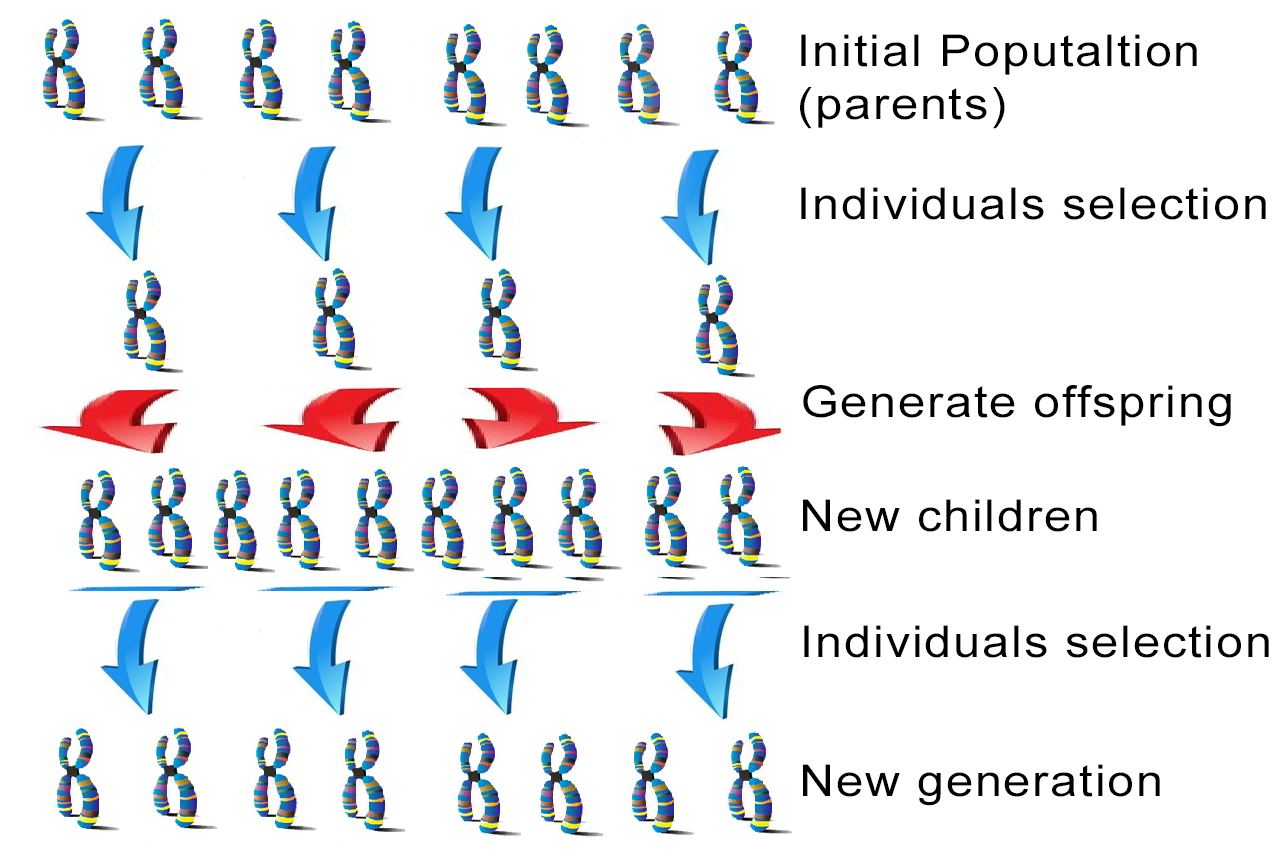
\includegraphics[width=\linewidth]{img/GA2selections.png}
  \caption{The 2  time for  the selection mode with the GA  mechanisme }\label{fig:GA2selections}
  \endminipage\hfill
\end{figure}
The last element to consider about the selection mode is when it is the more appropriate to use it? 
Indeed  the selection of the individual may intervene at 2 occasions (see figure \ref{fig:GA2selections}).  The first  the more conventional is  to select the parent  able to reproduce. The second is to select the children good enough for be part of the next generation. The interest of this is to be able to generate new children until the selection criteria are rich in order to have a population with acceptable children in sufficient quantity (This method is more efficient on the problem with lot of hard constraint). 


 

%idée 1 :  quesque le mode de selection  ...  
%			 c'est la method qui va etre utilisé pour choisire les individue qui pouron ce reprorduire.
%idée 3 le choix de ql selection est la plus aproprier
%			   le mode de selection impacte la qualité et la vitesse de la réponce 
%			   le mode choisie et fait en contion du problem a résoudre (pas de recette miracle) 
%
%idée 4  le mode de selection doit gardée une certaine variété  pour  avoir une convergence 
%			mais pas trop.
%			 
%idée 2  l'importantce de la selection 
%			 une population trop élitiste peu convergé prématuréméne 
%			  une selection trop peu restrictive peu empéché la convergence et l'optimisation

%idée 5  une multitude de mode de selection existe 123*
%
%idée 7 les modes de selection les plus comu et représentatif  
%
%idée6   la seleciton peut etre fait a plusier momen  64*
%			selection des parent
%			selection parmis les potentiel enfant les ql vous sourvivre 
	


%The selection mode have aim to pick-up the individual (or chromosome) the most interesting of the actual generation for build the next one.
% The individual chosen can be called parent, they reproduce to build the next generation.
%One of the difficult point is to understand who the more interesting individuals are from the actual generation. To this choice is essential because depending to the choice the quality of the answer and the convergence will be affect. 
%
%Among the goals of the selector is keep the variety and help to converge but for that is primordial to know the difference between the selections modes. Many mode was designed [123]* or adapted but some of they are more used and studied. Also the selection can be done at different time.  First for select the parent or after the crossover mutation and other operator for select the best children or even use both like is showed in [64]*.


%le role de la  selection 
%	\paragraph*{Elitist selection}
%	\paragraph*{Roulette wheel selection}
%	\paragraph*{Tournament selection}
%		\subparagraph{fonctionment}
%		\subparagraph{pool size}
%	
%%%%%%%%%%%%%%%%%%%%%%%%%%%%%%%%%%%%%%%%%%%%%%%%%%%%%%%%%%%%%%%%%%%%%%%%%%%
\subsubsection{Operators }


The operator have to aim the design of the next generation by generate the offspring. 
Once the parent able to the reproduction were selected (using the selection mode saw previously) it is time to engender a new children.
The techniques, to create a new population are numerous. Among them the more common  are the heritage (or selection), random generation, the crossover and mutation. 

\subparagraph{heritage or selection:}
The heritage or also called selection is a simple copy of the best parents to the next generation with no modification. This operator is commonly used to keep the best individual in order to do not lose the best solution if no upgrade is made by the other children. Indeed the other operator may propose degenerated children with is some time worst then their parents and the heritage  permit to conserve as is the individuals.
\\
The crossover and mutation have a more interesting mechanism. They are also the basis of many other customized operators and the understanding of the basic crossover and mutation required to use it.
 
 
\subparagraph{Crossover:} 

The crossover operator is directly inspired by the biologies. As 2 mammals reproduce to have progeny. Half of the genetic material of the two parents are used to create a child.
The crossover operator is mixing 2 individuals to create a new child. The aim of this is to merge 2 workable solutions to have one other solution potentially a bit better. To merge the 2 individuals it is existing many way like studied in \cite{113*mais2010}.
 
 \subparagraph{Mutation}
The mutation operator have to aim to add diversity by mutate some random allele of the chromosome. This mutation must be randomly choose and are useful to keep the diversity of the population. As the crossover different mutation are existing \cite{113*mais2010}. The mutation mechanism affect only rare genome in all the population. The genome mutated is randomly selected and the is will be based on random. 

\subparagraph*{Customized operators}
This 2 principals operators need to be choose carefully and in most of the case redesigned.
The redesign of the operator is essential in many occasion.
One of the first reason to redesign part of the operator is to fit well to the problem. A example is the mutation redesigned to explore the search space with a logic of close neighbour as in \cite{68*muhlenbein1989}.\\
The second reason is link to the chromosome coding. Depending then the chromosome coding chosen (binary, combinatorics, real, ...) the operator have to be adapted. An example is to modify the mutation and crossover to preserve the genomes in the real coding. The same operator can not be used for combinatoric coding or binary.\\
The third is more rare but in some case the operator have to be adapted depending then the selection mode chosen. An example is  given in  \cite{65*thierens1994} with the crossover and the mutation for a elitist selection. \\
Also one other reason to redesign the operators is to have operator fitting  to some of the hard constraint to the problem. In order to have operator able to create children respectful to some hard constraint of the problems.


%redesign some operateur (mostly  crossover  and Mutation
%idee 1 : operateur redesigne to fit the problem
%idee 2 : operateur redesigne to fit the chromosome coding (pour ne pas coupe des gene  ) 
%idee 3 : operateur doive etre adapté au mode de selection  comme le crossover  avec une selection elitiste 65*
%idee 4 : redesign a operateur  pour respecter certaine des hard constraint
% In many case the crossover need to be designed or redesigned depending to the problem. 
% In order to have an adapted crossover  the chromosome coding is primordial. Depending then if the chromosome coding is binary,real or other the the crossover must be redesigned to respect the it. Also the  crossover should be redesigned  
% Also the crossover work differently if the chromosome are code as binary or real for example and the crossover should redesign depending to the problem, the coding and some time for some specific selections like for elitist recombination [65]*. Redesigned the crossover can be useful to have crossover respect the genome or to can directly have an operator generate a solution that respect some of the hard constraint. 
% Mutation custom
%  and some of them are specific to the coding of the chromosome because like the precedent operator presented the  coding  affect the implementation of the mutation and may redesigned depending to the problems and also be redesigned do explore the search space with a logic of close neibourgh  like in [68]*.\\


\subparagraph{Operators rate}
 An other important element to take in consideration after the choice of the operator and their implementation is  rate of each of then. 
The rate of an operator correspond to the usage percentage of the operator on the chromosome, higher the rate is,  more this operator will be used at each generation generation. 
In the mutation the rate can be globally understood as a chance to one an genome to be muted. 
Finding the  best rate for every operators became a real challenge. The best solution to find the appropriate  operators and their associate rate for a specific problem no other choice to try the couple combination of operators with different rate like in \cite{73*wright1991,71*grefenstette1986,133*schwefel1984}.\\

 To conclude on the operators, they are an important factor to evolve generation after generation.  The operator have to keep the diversity  in order to have an efficient converge (not premature and not to late). The question of the diversity introduce by the operator was been studied in  \cite{80*serpell2010,95*miller1995} \cite{113*mais2010}. 
 It is appearing one good static configuration to keep diversity \cite{64*matsui1999} of chromosome is to have crossover mutation with height rate of crossover and small rate of mutation. 
But the rate of the operator can be adapted depending then the searched space, the convergence and other element. Some research was done on adapted the dynamically the rate of the operator depending too many external factor or using probability like is discussed in  \cite{110*eiben2003,133*schwefel1984,94*srinivas1994}


	
%%%%%%%%%%%%%%%%%%%%%%%%%%%%%%%%%%%%%%%%%%%%%%%%%%%%%%%%%%%%%%%%%%%%%%%%%%%%
\subsubsection{Setting and  set-up} \label{sec:Setting and  set-up}

The previous section introduce the different aspect of the GA and give the key to understand the different element and the mechanism of the genetic algorithm. Besides the GA explication is appear many primordial  choice  to set-up properly the algorithm. Part of their choice are interdependent and the connection between the different parameter can make the set-up tricky.
Also the GA has been studied for decades and many variant were developed over the time to make the GA more efficient. That give even more choice but no general set-up have been formulated.
To evaluate the  performance of a set-up the quality of this answer is used but also the speed of convergence in term of number of generation, and also the variety of the chromosome at each generation until the convergence. 
The variety is one of the factor useful to explain the convergence speed and the answer quality.
The variety is almost opposite of the convergence. It is when the chromosome  are all very different in the same generation but also generation after generation. A high variety is ideal at the beginning because this allows the optimization browse the search space and potentially help to jump the local minima. 
 As example if the finally solution is lock in a local minima after a to fast convergence that mean not enough variety has been introduce during the optimisation.

During the choice of the ideal parameters for GA the variety is a important element to preserved and more at the beginning of the optimisation to browse the search space.\\
 
However the GA stay complex to configure because of all this parameter to have a good answer quality in a reasonable period of convergence. Many aspect need to be adapted depending to the problem, constraint, size of the search space and … .   
Using the simple GA that mean configure a set of parameter. The parameter can be formalized as a vector like in \cite{71*grefenstette1986}. This formulation is especially  efficient test numerous setting. 
To set-up properly a GA few question need to be posed as in the table \ref{tab:GAsetting} and few setting must be test as in \cite{73*wright1991,71*grefenstette1986,133*schwefel1984}.

		
 \begin{table}
   \begin{tabular}{ | m{0.35\linewidth} | m{0.64\linewidth} |  }
     \hline
      \Emph{Inspiration or group}   & \Emph{ Algorithm}    \tabularnewline \hline 
	 Coding chromosome: & what coding choice? ( binary, combinatoric, real,...)				  	    \tabularnewline \hline 
	  Cost function.		 & How quantify the answer quality?		\tabularnewline  \hline  
	Population	: 			 & What size?  	    					\tabularnewline \cline{2-2}  
							 & What initialisation? (random or heuristic) \tabularnewline \hline  
	  Selection mode      	 & what choice of selection mode? 				 	    \tabularnewline \cline{2-2}
        				 	 & And depending then the mode chosen what set-up? \tabularnewline \cline{2-2}
        					 & As for tournament selection the size pool, the wheel repartition for roulette wheel or the number of parent selected for elitist...  	\tabularnewline \hline
      						 & What operators to use?	  	  		\tabularnewline \cline{2-2}
      	operators			 &	What implementation choice (customized operator or not)?	\tabularnewline \cline{2-2}
      						 &	What rate for each operators? 	 	  	\tabularnewline \hline
 Stopping criteria	 &	What stopping criteria to use? 									\tabularnewline \cline{2-2} & If  is  not by convergence what are the boundary?\tabularnewline  \hline  
   \end{tabular} \caption{Sumarizing the question to ask to configure the GA } \label{tab:GAsetting}
 \end{table}
%		coding : coding choice ( binary, combinatoric, real,...)\\
%		cost function    
%		population: size\\
%					initialisation\\
%		selection mode : 
%					choice of the selection mode \\
%						depending then the mode chosen the size of the pool, the wheel repartition, the number 							of parent selected...
%					
%		operators :  choice \\
%					implementation choice ( customized operator or not)\\
%					rate of each\\
%		also the stopping criteria 


%%%%%%%%%%%%%%%%%%%%%%%%%%%%%%%%%%%%%%%%%%%%%%%%%%%%%%%%%%%%%%%%%%%%%%%%%%%




